\section{Lower Bounds} \index{lower bound} \index{model of computation} \index{comparison model}

So far, we have been talking almost exclusively about how we can use different algorithms and data structures to solve certain problems as fast as possible. In this part, we will focus on proving certain problems cannot be solved as quickly as we might want. In other words, there is a limit to how good we can do. For example, in a comparison model, sorting can only be achieved at best in $\Omega(n \log n)$ time in the worst case.

Let $T_A(X)$ be the running time of algorithm $A$ given input $X$. Then, the worst-case running time is
$$
T_A(n) = \max_{|X|=n} T_A(X)
$$

The worst-case complexity of a \textbf{problem} $\Pi$ is the worst-case running time of the fastest algorithm for solving it. 
$$
T_{\Pi}(n) = \min_{\text{$A$ solves $\Pi$}} T_A(n) = \min_{\text{$A$ solves $\Pi$}} \max_{|X|=n}T_A(X)
$$

We can prove the upper-bound of the complexity of a problem by giving a specific algorithm $A$ that solves $\Pi$, and faster algorithms give us smaller (tighter and better) upper bounds.

However, to prove that a problem has a certain lower bound, we have to show that every algorithm that solves $\Pi$ has a worst-case running time $\Omega(f(n))$, or equivalently, that there is no algorithm that solves $\Pi$ that runs in $o(f(n))$ time. To be more specific, we need to specify what kinds of algorithms we want to consider, which is formally known as model of computation. For example, the comparison model is one model that is used to solve sorting and searching problems.

\section{Comparison Model}

In the comparison model, we consider all input items as black boxes, or more precisely, ADTs. The only operations allowed on the items are comparisons: $<, \leq, >, \geq, =$. Most searching and sorting algorithms we have been looking at so far use the comparison model: heap sort, merge sort, binary search and binary search tree, etc. In the comparison model, we count the number of comparisons and define it as the time cost of the algorithm.

\section{Decision Tree}

\subsection{Intuition}

Any comparison algorithm can be viewed as a tree of all possible comparisons, the outcomes of the comparisons, and the resulting answer. This tree is called a decision tree.

For any particular $n$,
\begin{itemize}
    \item \textit{internal node} corresponds to binary decision in the algorithm (in this case, binary comparisons)
    \item \textit{leaf} corresponds to a possible answer of the problem
    \item \textit{root-to-leaf path} corresponds to an execution of the algorithm
    \item \textit{length of the root-to-leaf path} corresponds to the time cost of the execution associated with that path
    \item \textit{height of the tree} (or depth of the deepest leaf) corresponds to the worst-case running time.
\end{itemize}

\subsection{Decision Tree for Searching}

In this subsection, we will look at the decision tree for binary search and use it to prove that the lower bound of searching under the comparison model is $\Omega(\log n)$.

\hfill

\begin{figure}[htbp]
    \centering
    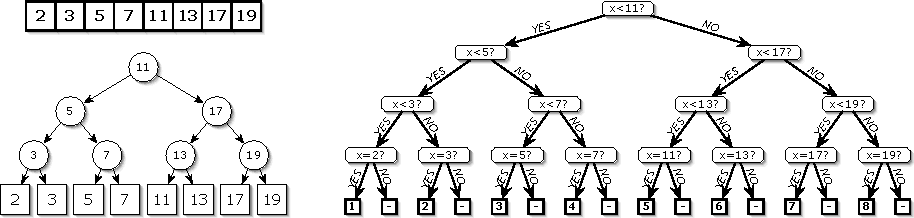
\includegraphics[width=\linewidth]{figures/binary_search_decision_tree.pdf}
    \caption{<caption>}
\end{figure}

\subsection{Decision Tree for Sorting}

\section{Sorting in Linear Time}